\section{Introduction}
\label{sec:intro}

Supercompilation is a semantics-driven program transformation technique based on symbolic evaluation (driving), constructor case analysis, generalisation, and fold/refold via memoisation.
Despite decades of development for functional languages, there is no widely accepted exposition of supercompilation for a dependently typed core language, where types depend on terms and where transformation steps must preserve typing and observational meaning.

This paper proposes a proof-theoretic account: \emph{supercompilation can be presented as focused cyclic sequent proof search} for a CoC-style dependent calculus with inductives.
The correspondence is meant to be exact at the level of operational moves: driving steps are invertible (asynchronous) sequent steps, case-splitting is a synchronous rule, and folding is cyclic closure via back-links.

\paragraph{Contributions.}
\begin{itemize}[leftmargin=*]
\item A concrete CoC-with-inductives term calculus recap (Section~\ref{sec:calculus}).
\item A focused cyclic sequent calculus designed to mirror supercompilation moves (Section~\ref{sec:focused}).
\item A precise operational dictionary between drive/split/fold and local sequent steps (Section~\ref{sec:sc-as-search}).
\item A proof-engineering perspective on \emph{post-hoc} induction principles: cyclic derivations allow the induction scheme to emerge from the discovered cycle structure (Section~\ref{sec:thesis:cyclic}).
\item A mechanisation status report for the Coq development (Section~\ref{sec:mech}).
\end{itemize}

\paragraph{Outline.}
Section~\ref{sec:thesis:pipeline} states the central thesis as a pipeline of four claims.
Sections~\ref{sec:calculus}--\ref{sec:focused} define the source calculus and the focused cyclic sequent system.
Section~\ref{sec:sc-as-search} presents worked correspondences.
Section~\ref{sec:related} discusses related work, and Section~\ref{sec:equiv} gives the formal equivalence statements.

\subsection{Main result pipeline}
\label{sec:thesis:pipeline}

\begin{center}
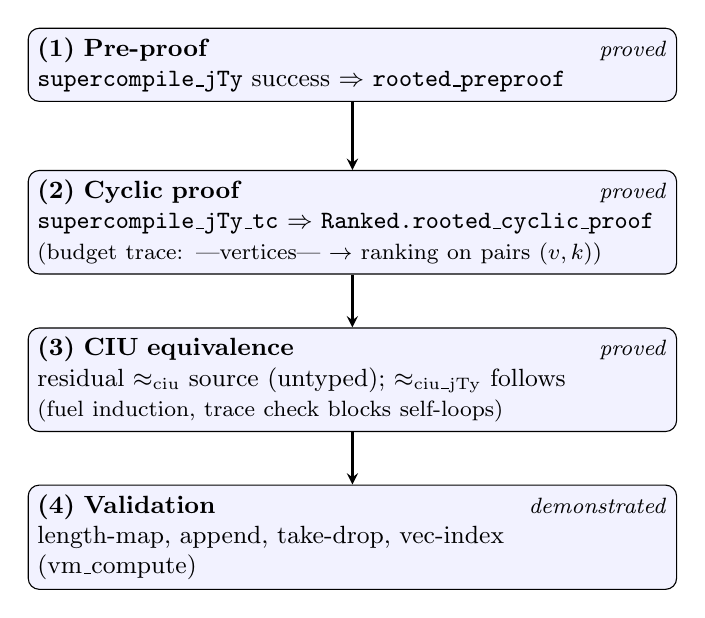
\begin{tikzpicture}[
  node distance=2cm,
  box/.style={rectangle,draw,rounded corners,text width=8cm,align=left,font=\small,fill=blue!5},
  arrow/.style={->,>=stealth,thick}
]
\node[box] (p1) {\textbf{(1) Pre-proof} \hfill {\footnotesize\textit{proved}} \\
  \texttt{supercompile\_jTy} success $\Rightarrow$ \texttt{rooted\_preproof}};
\node[box,below of=p1] (p2) {\textbf{(2) Cyclic proof} \hfill {\footnotesize\textit{proved}} \\
  \texttt{supercompile\_jTy\_tc} $\Rightarrow$ \texttt{Ranked.rooted\_cyclic\_proof} \\
  {\footnotesize (budget trace: |vertices| $\to$ ranking on pairs $(v,k)$)}};
\node[box,below of=p2] (p3) {\textbf{(3) CIU equivalence} \hfill {\footnotesize\textit{proved}} \\
  residual $\approx_{\mathrm{ciu}}$ source (untyped); $\approx_{\mathrm{ciu\_jTy}}$ follows \\
  {\footnotesize (fuel induction, trace check blocks self-loops)}};
\node[box,below of=p3] (p4) {\textbf{(4) Validation} \hfill {\footnotesize\textit{demonstrated}} \\
  length-map, append, take-drop, vec-index (vm\_compute)};

\draw[arrow] (p1) -- (p2);
\draw[arrow] (p2) -- (p3);
\draw[arrow] (p3) -- (p4);
\end{tikzpicture}
\end{center}

The four claims form a dependency chain: each tier builds on the previous. All are mechanized in Coq with full proofs (0 axioms, 0 admitted lemmas).

\paragraph{Claim 1: Supercompilation yields a pre-proof.}
When the supercompiler succeeds on a well-typed input, the resulting configuration graph directly forms a \emph{rooted pre-proof}.
Every vertex is labelled with a judgement and satisfies its local sequent rule; every successor is a valid vertex; and the edge structure corresponds exactly to the drive/split/fold operations of the supercompiler.
This claim is \textbf{mechanized} in Coq via $\texttt{all\_supercompiled\_programs\_yield\_preproof}$ (\texttt{SupercompilationCorrespondence.v:1659}) and the three graph-level correspondence lemmas (\texttt{drive\_corresponds\_to\_async\_edge}, \texttt{split\_corresponds\_to\_sync\_edge}, \texttt{memo\_corresponds\_to\_fold}).
See Section~\ref{sec:equiv} for the formal statement (Theorem~\ref{thm:pre-proof}).

\paragraph{Claim 2: Termination yields a cyclic proof.}
A pre-proof becomes a \emph{cyclic proof} when it additionally satisfies a global progress condition: every cycle must contain at least one progress edge (a case-split on a neutral scrutinee), and there exists a well-founded ranking that strictly decreases along progress edges.
The supercompiler enforces this via a trace-condition check during graph construction.
We prove this by constructing a budget-instrumented trace graph: vertices are lifted to pairs $(v,k)$ where $k \in [0, B]$ is a budget counter consumed on progress edges and preserved on non-progress edges.
The resulting trace graph is acyclic, yielding a full $\mathsf{ranking\_condition}$ with rank $\lambda(v,k).\,k$.
This claim is \textbf{mechanized}: $\texttt{supercompile\_yields\_rooted\_cyclic\_proof}$ (\texttt{SupercompilationCorrespondence.v}).
See Section~\ref{sec:equiv} for the formal statement (Theorem~\ref{thm:cyclic-proof}).

\paragraph{Claim 3: Cyclic proofs imply CIU equivalence.}
The ultimate soundness guarantee is \emph{contextual equivalence} (CIU): the program read off from a valid cyclic proof should be observationally indistinguishable from the original source program under all closing substitutions.
This claim is \textbf{mechanized}: $\texttt{supercompile\_ciu\_soundness\_untyped}$ and $\texttt{supercompile\_ciu\_soundness\_typed}$ (\texttt{SupercompilationCorrespondence.v}) by fuel induction. The trace condition prevents self-loops that would introduce non-termination.
See Section~\ref{sec:equiv} for the formal statement (Theorem~\ref{thm:ciu}).

\paragraph{Claim 4: The pipeline obtains for our examples.}
The framework is validated on a suite of standard supercompilation examples (length-map fusion, append length normalisation, take-drop, etc.).
For each example, the supercompiler produces a residual, and computational equality with the expected result is verified by $\mathtt{vm\_compute}$ in Coq (\texttt{Equiv/SupercompileChecklistIndexPipeline.v}).
See Section~\ref{sec:equiv} for the formal statement (Proposition~\ref{prop:examples}) and Section~\ref{sec:example} for a detailed walkthrough.

\subsection{Why focusing matters}
Focusing separates proof search into an \emph{asynchronous} (invertible) phase and a \emph{synchronous} (choice-bearing) phase.
This mirrors supercompilation practice:
\begin{itemize}[leftmargin=*]
\item Driving is largely deterministic (invertible phase).
\item Generalisation and folding are the essential choice points (synchronous phase).
\item Case-splitting sits at the boundary: it is forced when the scrutinee is neutral, but introduces branching.
\end{itemize}

\subsection{Why cyclic proofs matter: post-hoc induction principles}
\label{sec:thesis:cyclic}

A crucial advantage of the cyclic proof framework is that it allows the \emph{induction principle to emerge during proof search} rather than requiring it to be specified upfront. This is fundamentally different from traditional inductive proof systems.

\textbf{Traditional induction:} In standard natural deduction or sequent calculus for inductive types, the induction principle must be chosen at the start of the proof. For example, to prove a property about lists, one typically applies structural induction on the list, which commits to a specific recursive structure immediately. If the property requires a different induction scheme (e.g., on a different variable, or on a measure combining multiple arguments), the proof fails and must be restarted with a new principle.

\textbf{Cyclic induction:} In the cyclic proof setting, we instead:
\begin{enumerate}
\item Begin with the goal sequent (no induction principle required)
\item Drive and split as needed, following the term structure
\item Form backlinks when we encounter goals that match previous vertices
\item The induction principle is \emph{read off} from the completed cyclic proof graph
\end{enumerate}

The key insight is that the cycle structure itself \emph{is} the induction principle. The trace condition (ensuring structural descent through progress events) guarantees soundness, but the actual induction scheme---which variables are analyzed, in what order, and with what invariants---emerges naturally from the proof search process.

\textbf{Connection to supercompilation:} This matches exactly how supercompilation works: the residual program's recursive structure is discovered by the driving process, not prescribed in advance. When the supercompiler folds a configuration back to an earlier one (via memo table lookup), it has implicitly discovered a valid recursion scheme.

\textbf{Example:} Consider proving that $\texttt{length (map f l)}$ equals $\texttt{length l}$. A traditional proof requires choosing to induct on $l$ at the outset. In the cyclic/supercompilation setting, after driving and splitting we encounter a subgoal $\texttt{length (map f xs)}$ which matches the original goal under substitution $l \mapsto xs$, yielding a backlink and thus an induction scheme discovered post-hoc.
